\chapter{Kubernetes}\label{ch:kubernetes}

\section{Overview}

Kubernetes is a container platform for high availability clusters.
There exist plugins for integration tests for Kubernetes with the name kubetest\footnote{\url{https://kubetest.readthedocs.io/en/latest/}}. They contain conformance tests, as well as e2e tests (end-to-end).
That can be all built and executed on the system. Therefore, a Dockerfile for setting up Kubernetes is necessary. The challenge is, that 2 big Github repositories have to be cloned and integrated into the docker image. These are using a lot of space. One solution is using a self-developed multi staging Dockerfile\footnote{\url{https://github.com/s390x-container-samples/s390x-kubernetes-test/blob/master/Dockerfile}}. 
So 2 different Dockerfiles are used in one Dockerfile and one of them is required for building. The other one is applied for the installation and upgrading to a special version. At the end the size of the Docker image has got only the size of the child image regardless of the repository size in the parent Dockerfile.
Additionally, a Dockerfile for executing tests based on the Kubernetes Docker image has to be written.

\section{Docker Multi-Arch Image}
As mentioned in \ref{Docker-Intro} "Introduction of Docker", Docker is integrated as a base container engine for Kubernetes tests by the community. \\  
Docker Inc. is maintaining a Docker image with the name "Docker-in-Docker" for multiple architectures, incl. s390x. 
This Docker image was introduced by the Docker contributor Jerome Petazzoni (Tianon) with the name dind\footnote{\url{https://github.com/jpetazzo/dind}}. Docker can be installed on Ubuntu, openSUSE, Fedora, ArchLinux and Alpine on this way.
The base Docker image on Docker Hub\footnote{\url{https://hub.docker.com/_/docker}} is based on Alpine Linux.
The base image for a specified architecture can be integrated with 2 methods. Firstly, the s390x base image can be pulled to the local container registry with \textbf{docker pull s390x/docker}. The specification \textbf{docker} behind pull alone would download the Docker image for the host architecture or would choose the platform for a multi-arch build with the platform option of BuildX in the command \textbf{docker build}. The prefix \textbf{s390x} before docker specifies a specific available architecture. 
The second option is the integration of \textbf{s390x/docker} into the FROM command inside of the Dockerfile. Both methods are downloading the latest Docker version with Ubuntu from \path{docker.io/s390x/docker:latest} and register this Docker image in the local registry.
Therefore, this image is used as a base image in the self-developed Dockerfile for Kubernetes.



\section{Multi-Staging Dockerfile}

A multi-staging Dockerfile is using different systems in one Dockerfile for different stages. These systems are receiving special names as indicators with "AS" behind the "FROM" with the base image name. 
Default this feature is applied for building applications in one stage and executing the copied application in another stage. The same counts for cloning Github repositories and building binary files based on it. On this way, a lot of space is saved.
Concluding, the docker image has got only the size of the executing system with the application file (without all the code). 
That is an "experimental feature"  at the moment. Therefore the \textbf{experimental flag} is necessary to export or set before operating (see \ref{Multi-Architecture-Images} "Multi-Architecture Images"). \\
Default one image is receiving the name build and the other one a name of how it will be applied. In our case, the second image has got the name work. 
The second image is copying with "COPY --from=build" all required built data from the first image. Therefore, it can be used for running the application. 
On this way, it is possible to reduce the size of a docker image. \\
Multi-staging Dockerfiles are an approved method for executing binaries based on Github repositories.


\section{Installation}

Kubernetes requires a lot of packages for running and for tests. These will be installed together with the RUN command.
Build is the name of the parent Dockerfile to be able to copy needed files and directories from there.
Docker is pre-installed with the base Docker image in the FROM command. This base is required for a successful installation of Kubernetes. \\
A Dockerfile is installing only necessary packages and includes packages of the base image. Therefore, curl, git and gnupg have to be installed first for the following installation.
Afterwards, the packages kubelet and kubeadm can be installed in the parent Dockerfile for working with Kubernetes. \textbf{Docker} in the base image contains the container engine docker with all docker commands. CRI/O or containerd would be allowed, too. 
The Docker daemon will be used because that is the main used container engine of the Kubernetes project and all tests are running with it. \\ 
\textbf{Kubelet} is the primary node agent running on each node and is responsible for different runnable containers in a pod. Pods are deployable units defined in JSON or a yaml file. This feature is used for \ref{Kub-IntegrationTest} "integration tests" in the CI/CD pipepline.
Pods include a single or a group of containers with shared storage and network resources. Hosting of distributed systems  with different services in different containers can work together. Consequential one pod is something as one "logical host". \\
\textbf{Kubeadm} is the administration tool to set up clusters. It is necessary to upgrade Kubernetes to other versions. Clusters can be initialized. The network can be configured and the command \textbf{kubectl} (Kubernetes Control Plane) for adding additional nodes to a cluster can be initialized. 

\begin{figure}[H]
\centering
\begin{boxedverbatim}
FROM s390x/ubuntu:18.04 AS kub-build
 
# The author
MAINTAINER Sarah Julia Kriesch <sarah.kriesch@ibm.com>

#Installation
RUN echo "Installing necessary packages" && \
apt-get update && apt-get install -y \
apt-transport-https \
apt-utils \
systemd \
curl \
git \
ca-certificates \
gnupg-agent \
software-properties-common \
&& curl -s https://packages.cloud.google.com/apt/doc/apt-key.gpg | apt-key add - \
&& echo "deb https://apt.kubernetes.io/ kubernetes-xenial main" \
> /etc/apt/sources.list.d/kubernetes.list \
&& apt-get update && apt-get install -y \
docker.io \
kubelet \
kubeadm \
&& apt-mark hold kubelet kubeadm kubectl \
&& apt-get clean \
&& rm -rf /var/lib/apt/lists/* /tmp/* /var/tmp/* \
&& systemctl enable docker 
\end{boxedverbatim}
 \caption{Kubernetes Installation}
    \label{kubernetes-installation}
\end{figure}

\section{Installation of the Latest Go}

There were some issues with older Go versions as 1.10 during building tests for Kubernetes. Therefore a higher version (min. 1.13) should be used. It is recommended to use the latest Go version for last versioned Kubernetes tests. It is possible to receive the version number of the last Go release with the command \\ 
\lstinline!curl https://golang.org/VERSION?m=text!. \\ 
This version number has to be included before linux-s390x.tar.gz for downloading the special s390x archive from the Go directory by \url{dl.google.com}. Then the version number has to be called with curl inside of another curl command with the whole path to the special tar archive on \url{dl.google.com}. Every tar archive has got the same structure for every version (\lstinline!$version.$architecture.tar.gz!). On this way the latest version of Go is integrable into the curl command that it can be installed. Directories for bin, pkg and src have to be created after extracting this tar archive in the \path{/root/} directory. They are not integrated in the tar archive. \\

The environment variables for GOROOT, GOPATH and PATH have to be set with ENV on the top of the Dockerfile for successful builds later. PWD is added because Github repositories have to be cloned to this directory. \\

The ENV variables will be on the top of the Dockerfile. The part for the "Installation of Go" will be attached to the end of the Kubernetes installation part.

\begin{figure}[H]
\centering
\begin{boxedverbatim}
ENV GOROOT=/root/go
ENV GOPATH=/root/go
ENV PATH=$GOPATH/bin:$PATH
ENV PATH=$PATH:$GOROOT/bin
ENV PWD=/root/go/src/

#Installation of latest GO
&& echo "Installation of latest GO" && \
curl "https://dl.google.com/go/ \
$(curl https://golang.org/VERSION?m=text).linux-s390x.tar.gz" \
| tar -C /root/ -xz \
&& mkdir -p /root/go/{bin,pkg,src} 
\end{boxedverbatim}
 \caption{Go Installation}
    \label{go-installation}
\end{figure}

\section{Installation of special Kubernetes Versions}

The Dockerfile should be usable for tests of different Kubernetes versions. Therefore, the feature of a changeable version number is added with \lstinline!ARG VERSION=v1.19.2!. This release version is adaptable with \\
\verb+--build-arg VERSION=$KUBERNETES_VERSION+ \\
in the build command of \textbf{docker buildx}.
Jenkins and Prow are working both with executable scripts. The Kubernetes version can be handled as a variable for all required Docker builds.
Default, the version of a special software and with it the branch can be chosen in the CI/CD system. Afterwards, the special software version has to be installed. In this case, the build command is receiving the variable for the installation. These verian numbers are used as tags in Github. So one special tagged branch can be chosen during \textbf{git clone} with \verb+--branch ${VERSION}+.
The Kubernetes project is providing a special Kubernetes installation for "Kubernetes in Docker" in their repository \textbf{kubernetes/kubernetes}.
After the checkout of the chosen release inside of a working Go environment, \verb+CMD make release-in-a-container ARCH=s390x+ is installing Kubernetes for the architecture s390x inside of a Docker container. \\
This command is integrated into the parent Dockerfile with the Go environment. The version number is additionally used for the test Docker image.


\section{Conformance Tests}

Some problems appeared during the build of the static e2e.test file with Go inside of a Docker image. 
Default the repository \textbf{test-infra} contains all tests for Kubernetes provided by the community. 
These can be used of course and are updated continuously. That is the reason that a separate e2e.test exist for every version. Inside of this test-infra directory kubetest can be installed with \textbf{go install}. 
That is downloading all available Kubernetes tests. So you can use them to test the own Kubernetes cluster and the used software. \\

The test Kubernetes Dockerfile\footnote{\url{https://github.com/s390x-container-samples/s390x-kubernetes-test/blob/master/test/Dockerfile}} has integrated the download of a tar archive with a static e2e.test file and all required Go frameworks as ginkgo.
These tests can be found under \path{/root/kubernetes/test/bin/} then. That includes conformance tests.
The name of the most relevant tests for the Kubernetes community is "conformance tests". These conformance tests are executed with e2e.test  which can be built with make inside of the kubernetes repository. 
In this case a static e2e.test file is used for every Kubernetes version inside of the test Docker image together with all required Go frameworks. These tests certify the software to comply regular standards. Only with complying these standards, Kubernetes software is allowed to become Kubernetes certified\footnote{\url{https://github.com/cncf/k8s-conformance}}. 

Conformance tests are testing all dependencies with other cloud providers or with additional software. The following command is used to integrate conformance tests. \\
\verb+e2e.test --kubeconfig /etc/kubernetes/admin.conf --provider local \+ \\
\verb+-ginkgo.focus="\[sig-network\].*Conformance" -num-nodes 1+  \\
The \textbf{local} behind provider identifies that all tests should run only local at the moment. That has the reason that the QEMU command has to be adapted with network configurations and open ports for communication for these features.
The \textbf{gingo.focus} includes conformance tests.


\subsection{End To End Testing}
The e2e.test suite is a end-to-end testing framework for Kubernetes. It is testing Kubernetes for all required functionality \cite{Ohly2019}. This framework is written in Go and is using the Ginkgo Testing framework\footnote{\url{https://onsi.github.io/ginkgo/}} for expressive and comprehensive tests with the style of Behavior Driven Development (BDD).
Expected behaviors are described in specs inside of the Kubernetes directory for e2e-tests\footnote{\url{https://github.com/kubernetes/kubernetes/tree/master/test/e2e}}. These tests exist for every Kubernetes version in specified Github branches. \\
The test is built with the installed Go based on the file \textbf{e2e\_test.go}. Kubernetes has been importing all multiple providers, in-tree tests, configuration support, and bindata file lookup in the file e2e\_test.go.
The vendoring code and their dependencies are available under \path{k8s.io/kubernetes/vendor/}. Additionally, these can be tested limited to necessary dependencies. \\
Conformance tests can be included with: \\
\begin{figure}[H]
\centering
\begin{boxedverbatim}
FROM kubernetes

ARG VERSION=v1.19.2

ENV KUBECONFIG=/etc/kubernetes/admin.conf
ENV KUBERNETES_CONFORMANCE_TEST=y

RUN echo "Download of e2e.test"  \
    && curl "https://storage.googleapis.com/kubernetes-release/release/ \
    ${VERSION}/kubernetes-test-linux-s390x.tar.gz" | tar -C /root/ -xz \
    && cd /root/kubernetes/test/bin/
CMD e2e.test --kubeconfig /etc/kubernetes/admin.conf --provider skeleton \
-context kind-kind -ginkgo.focus="\[sig-network\].*Conformance" -num-nodes 1 
\end{boxedverbatim}
 \caption{E2e-Test}
    \label{e2e-test}
\end{figure}

These conformance tests are a subset of e2e-tests \cite[~p.8]{Omichi2018}. Every vendor is receiving a certification by Kubernetes with passing all required conformance tests. 167 of 999 tests had been such conformance tests in the year 2018 \cite[~p.9]{Omichi2018}.
A working Kubernetes test setup is required for running tests against it.


\section{Integration Tests} \label{Kub-IntegrationTest}

It is possible to execute \ref{TestLevel} "integration tests" for Kubernetes in Prow and Jenkins.
The Kubernetes community has got a test team with the name Sig-Testing. They are developing tests for Kubernetes continuously. Therefore integration tests for Prow are available on Github\footnote{\url{https://github.com/kubernetes/test-infra/blob/master/config/jobs/kubernetes/sig-testing/integration.yaml}}. This test file can be integrated into Jenkins via the Kubernetes plugin\footnote{\url{https://github.com/jenkinsci/kubernetes-plugin}}, too.

Jenkins can deploy a specified Kubernetes cluster inside of a Docker image based on the requirements im the yaml file.

\section{Integration into CI/CD}

The Kubernetes project has been using Prow as a CI/CD system. Prow is a Kubernetes based CI/CD system further developed based on Jenkins \cite{JAXenter}. That implifies, that the existing CI/CD pipeline can work only with containers.
Before the integration into the community pipeline, it is possible to use a default Jenkins system with an integrated Kubernetes plugin because of identical configuration files. An additional advantage in this case is the chance to test the integration of Kubernetes into QEMU before providing the IBM Z environment container based for test purposes.

\begin{figure}[H]
\centering
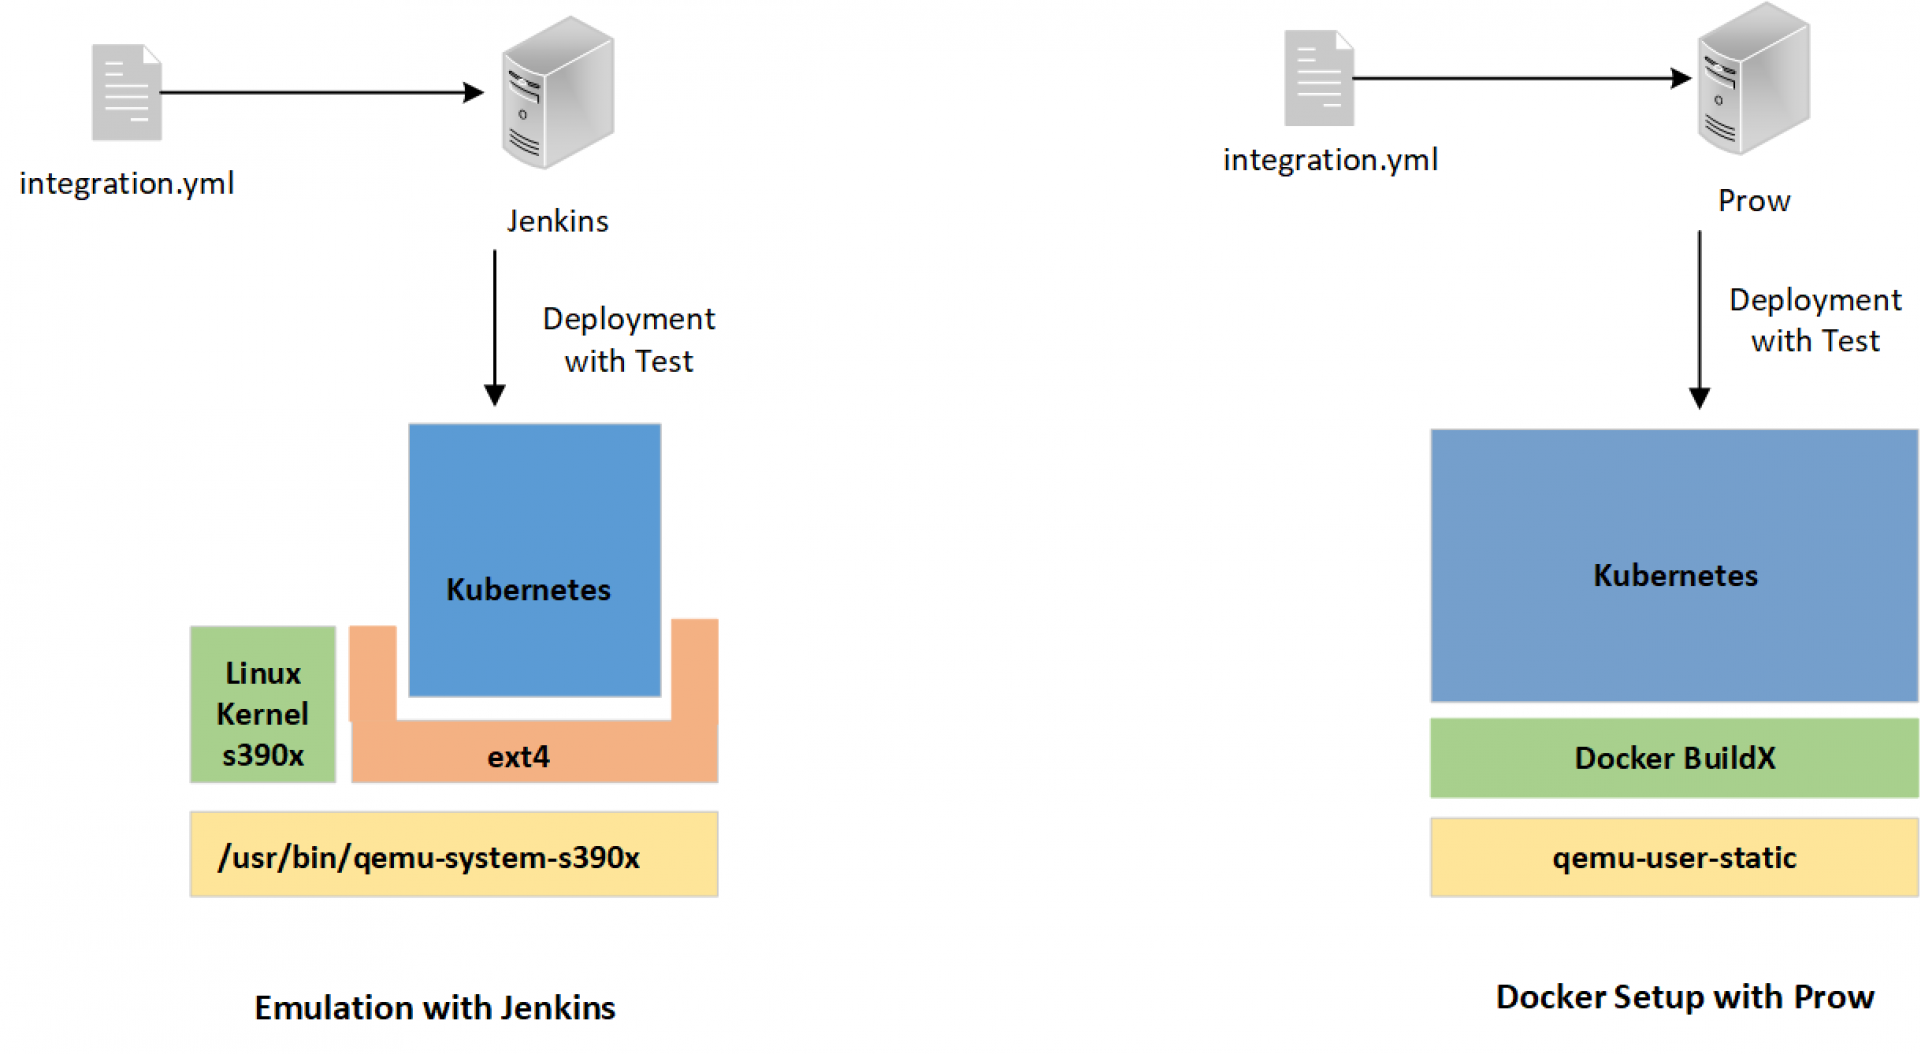
\includegraphics[height=8cm, width=12cm]{Jenkins-versus-Prow}
 \caption{Jenkins versus Prow}
    \label{JenkinsProw}
\end{figure}


\subsection{Jenkins versus Prow}

As mentioned in \ref{CI-CD} "CI/CD Systems", \textbf{Jenkins}\footnote{\url{https://www.jenkins.io/}} is the most popular open-source CI/CD system. This open-source project has started with a default CI/CD workflow based on real hardware and later on virtual machines to test software before the release. Jenkins provides many plugins\footnote{\url{https://plugins.jenkins.io/}} for git integration about release management support until container deployments. \\
There exists a special \textbf{Kubernetes plugin}\footnote{\url{https://plugins.jenkins.io/kubernetes/}}, that Jenkins can understand yaml configuration files for Kubernetes deployments which are used for integration tests by the Kubernetes community as an example. On this way, Jenkins can execute the same tests as Prow together with emulations because the Kubernetes environment is deployed inside of a emulated system. Jenkins can handle emulated systems the same as virtual machines. The Kubernetes plugin makes automated Kubernetes deployments possible. Therefore, a Jenkins installation is the best choice for the transition from emulated systems together with container technologies to a working test strategy with container based test environments in Prow.

\textbf{Jenkins X}\footnote{\url{https://jenkins-x.io/}} has been developed based on Jenkins specialized on Kubernetes and cloud native environments. That means, that something as the Kubernetes plugin is integrated and the system can work with public cloud providers and other cloud technologies for test and production deployment pipelines. All in all, Jenkins X is an improved version of Jenkins for cloud environments. The system can work with container registries, understands yaml configuration files without additional plugins and is able to deploy scalable systems based on containers in the local data centre as well as in the public cloud (AWS, Google Cloud, IBM cloud, Azure).

\textbf{Prow}\footnote{\url{https://jenkins-x.io/docs/reference/components/prow/}} is a Kubernetes-native solution based on Jenkins X. This CI/CD system is used by projects as Kubernetes, Istio und OpenShift which are all based on Kubernetes. This system is something as a Jenkins X expanded with special Kubernetes APIs and cloud specific features. It can understand and deploy only Kubernetes based environments. Other configurations are not supported. The benefit in comparison to Jenkins is, that yaml configurations for Kubernetes setups are transferable between Jenkins and Prow.

\subsection{System Requirements} \label{Kubernetes_Requirements}

Jenkins can include all required installation of integration tests and the whole system setup into the specified Docker image. Therefore, the disk image size can be defined based on the Docker image and the specified command in \ref{ExternalFile system} "Converting Docker Image to External File System" with \\
\lstinline!docker images | grep 'Kubernetes-Test' | awk '{print int($7+0.5)"G"}'! \\

The Kubernetes community is referencing\footnote{\url{https://kubernetes.io/docs/setup/production-environment/tools/kubeadm/install-kubeadm/\#before-you-begin}} a minimum about 2GB of memory and 2 CPUs per system. 
It has to be observerd, that Kubernetes is watching master and worker node as a own system. Both are on one system in our case. Additionally, some RAM and CPU should be added for running tests. Therefore, 6GB for memory and 5 CPUs will be calculated for the QEMU setup.

\subsection{Tests with Jenkins}

Both Docker images can be built with Jenkins. The Kubernetes plugin can read yaml files for deployments of pods.
Therefore, the Kubernetes base environment can be set up first and Jenkins can install the test environment for integration tests inside of the Docker image. The test Docker image is built in the next step based on this test environment.
Afterwards, the launch of the system with QEMU is executed.

In this step the QEMU image has to be prepared with the size of the Docker image \textbf{kubernetes-test}.
The file system of kubernetes-test has to be exported to a new directory \textbf{rootfs}.
Then the image has to be formatted with ext4 and this image is mounted in \path{/mnt/} as \textbf{rootfs}.
On this way, the content of the Docker image can be copied into the formatted QEMU image via \path{/mnt/rootfs/}.

\begin{figure}[H]
\centering
\begin{boxedverbatim}
qemu-img create -f raw cassandra-s390x.img $(docker images | grep 'kubernetes-test' \
| awk '{print int($7+0.5)"G"}')
docker export $(docker create kubernetes-test) | tar -C "rootfs" -xvf -
mkfs.ext4 -F kubernetes-s390x.img
mkdir /mnt/rootfs
mount -o loop kubernetes-s390x.img /mnt/rootfs
cp -r rootfs/* /mnt/rootfs/.
\end{boxedverbatim}
 \caption{Preparation of Kubernetes Rootfs}
    \label{Kubernetes-Rootfs}
\end{figure}

The command \textbf{debootstrap} can be used for fetching the signed Linux Kernel of Alpine Linux, too.
This command is the following: \\
\begin{boxedverbatim}
mkdir kernel-alpine
debootstrap --include=linux-generic --arch=s390x --variant=minbase v3.7 \
kernel-alpine https://pkgs.alpinelinux.org/ 
\end{boxedverbatim}

If the file system import was executed successfully, the emulation can be started in the next step with referenced \ref{Kubernetes_Requirements} "System Requirements".

\begin{figure}[H]
\centering
\begin{boxedverbatim}
 /usr/bin/qemu-system-s390x -kernel bzImage -m 40G -M s390-ccw-virtio -nodefaults \
 -device sclpconsole,chardev=console -parallel none -net none -chardev stdio, \
 id=console,signal=off,mux=on -mon chardev=console -nographic -smp 5 \
 -hda /kubernetes-test.img \
 --append 'root=/dev/vda rw console=ttyS0 rdinit=/bin/bash' 
\end{boxedverbatim}
 \caption{Run Kubernetes}
    \label{RunKubernetes}
\end{figure}
